\documentclass[11pt]{article}

\usepackage{fullpage}
\usepackage{amsmath, amssymb, bm, cite, epsfig, psfrag}
\usepackage{graphicx}
\usepackage{float}
\usepackage{amsthm}
\usepackage{amsfonts}
\usepackage{listings}
\usepackage{cite}
\usepackage{hyperref}
\usepackage{tikz}
\usepackage{enumerate}
\usepackage{xcolor}
\usepackage[outercaption]{sidecap}
\usetikzlibrary{shapes,arrows}
\usepackage{mdframed}
\usetikzlibrary{automata, positioning, arrows}
%\usetikzlibrary{dsp,chains}

%\restylefloat{figure}
%\theoremstyle{plain}      \newtheorem{theorem}{Theorem}
%\theoremstyle{definition} \newtheorem{definition}{Definition}

\def\del{\partial}
\def\ds{\displaystyle}
\def\ts{\textstyle}
\def\beq{\begin{equation}}
\def\eeq{\end{equation}}
\def\beqa{\begin{eqnarray}}
\def\eeqa{\end{eqnarray}}
\def\beqan{\begin{eqnarray*}}
\def\eeqan{\end{eqnarray*}}
\def\nn{\nonumber}
\def\binomial{\mathop{\mathrm{binomial}}}
\def\half{{\ts\frac{1}{2}}}
\def\Half{{\frac{1}{2}}}
\def\N{{\mathbb{N}}}
\def\Z{{\mathbb{Z}}}
\def\Q{{\mathbb{Q}}}
\def\F{{\mathbb{F}}}
\def\R{{\mathbb{R}}}
\def\C{{\mathbb{C}}}
\def\argmin{\mathop{\mathrm{arg\,min}}}
\def\argmax{\mathop{\mathrm{arg\,max}}}
%\def\span{\mathop{\mathrm{span}}}
\def\diag{\mathop{\mathrm{diag}}}
\def\x{\times}
\def\limn{\lim_{n \rightarrow \infty}}
\def\liminfn{\liminf_{n \rightarrow \infty}}
\def\limsupn{\limsup_{n \rightarrow \infty}}
\def\MID{\,|\,}
\def\MIDD{\,;\,}

\newtheorem{proposition}{Proposition}
\newtheorem{definition}{Definition}
\newtheorem{theorem}{Theorem}
\newtheorem{lemma}{Lemma}
\newtheorem{corollary}{Corollary}
\newtheorem{assumption}{Assumption}
\newtheorem{claim}{Claim}
\def\qed{\mbox{} \hfill $\Box$}
\setlength{\unitlength}{1mm}

\def\bhat{\widehat{b}}
\def\ehat{\widehat{e}}
\def\phat{\widehat{p}}
\def\qhat{\widehat{q}}
\def\rhat{\widehat{r}}
\def\shat{\widehat{s}}
\def\uhat{\widehat{u}}
\def\ubar{\overline{u}}
\def\vhat{\widehat{v}}
\def\xhat{\widehat{x}}
\def\xbar{\overline{x}}
\def\zhat{\widehat{z}}
\def\zbar{\overline{z}}
\def\la{\leftarrow}
\def\ra{\rightarrow}
\def\MSE{\mbox{\small \sffamily MSE}}
\def\SNR{\mbox{\small \sffamily SNR}}
\def\SINR{\mbox{\small \sffamily SINR}}
\def\arr{\rightarrow}
\def\Exp{\mathbb{E}}
\def\var{\mbox{var}}
\def\Tr{\mbox{Tr}}
\def\tm1{t\! - \! 1}
\def\tp1{t\! + \! 1}

\def\Xset{{\cal X}}

\newcommand{\bs}[1]{{\boldsymbol{{#1}}}}
\newcommand{\one}{\boldsymbol{1}}
\newcommand{\abf}{\boldsymbol{a}}
\newcommand{\bbf}{{\boldsymbol{b}}}
\newcommand{\dbf}{\boldsymbol{d}}
\newcommand{\ebf}{\boldsymbol{e}}
\newcommand{\gbf}{\boldsymbol{g}}
\newcommand{\hbf}{\boldsymbol{h}}
\newcommand{\pbf}{\boldsymbol{p}}
\newcommand{\pbfhat}{\widehat{\boldsymbol{p}}}
\newcommand{\qbf}{\boldsymbol{q}}
\newcommand{\qbfhat}{\widehat{\boldsymbol{q}}}
\newcommand{\rbf}{\boldsymbol{r}}
\newcommand{\rbfhat}{\widehat{\boldsymbol{r}}}
\newcommand{\sbf}{\boldsymbol{s}}
\newcommand{\sbfhat}{\widehat{\boldsymbol{s}}}
\newcommand{\ubf}{\boldsymbol{u}}
\newcommand{\ubfhat}{\widehat{\boldsymbol{u}}}
\newcommand{\utildebf}{\tilde{\boldsymbol{u}}}
\newcommand{\vbf}{\boldsymbol{v}}
\newcommand{\vbfhat}{\widehat{\boldsymbol{v}}}
\newcommand{\wbf}{\boldsymbol{w}}
\newcommand{\wbfhat}{\widehat{\boldsymbol{w}}}
\newcommand{\xbf}{\boldsymbol{x}}
\newcommand{\xbfhat}{\widehat{\boldsymbol{x}}}
\newcommand{\xbfbar}{\overline{\boldsymbol{x}}}
\newcommand{\ybf}{\boldsymbol{y}}
\newcommand{\zbf}{\boldsymbol{z}}
\newcommand{\zbfbar}{\overline{\boldsymbol{z}}}
\newcommand{\zbfhat}{\widehat{\boldsymbol{z}}}
\newcommand{\Ahat}{\widehat{A}}
\newcommand{\Abf}{\boldsymbol{A}}
\newcommand{\Bbf}{\boldsymbol{B}}
\newcommand{\Cbf}{\boldsymbol{C}}
\newcommand{\Bbfhat}{\widehat{\boldsymbol{B}}}
\newcommand{\Dbf}{\boldsymbol{D}}
\newcommand{\Gbf}{\boldsymbol{G}}
\newcommand{\Hbf}{\boldsymbol{H}}
\newcommand{\Kbf}{\boldsymbol{K}}
\newcommand{\Pbf}{\boldsymbol{P}}
\newcommand{\Phat}{\widehat{P}}
\newcommand{\Qbf}{\boldsymbol{Q}}
\newcommand{\Rbf}{\boldsymbol{R}}
\newcommand{\Rhat}{\widehat{R}}
\newcommand{\Sbf}{\boldsymbol{S}}
\newcommand{\Ubf}{\boldsymbol{U}}
\newcommand{\Vbf}{\boldsymbol{V}}
\newcommand{\Wbf}{\boldsymbol{W}}
\newcommand{\Xhat}{\widehat{X}}
\newcommand{\Xbf}{\boldsymbol{X}}
\newcommand{\Ybf}{\boldsymbol{Y}}
\newcommand{\Zbf}{\boldsymbol{Z}}
\newcommand{\Zhat}{\widehat{Z}}
\newcommand{\Zbfhat}{\widehat{\boldsymbol{Z}}}
\def\alphabf{{\boldsymbol \alpha}}
\def\betabf{{\boldsymbol \beta}}
\def\mubf{{\boldsymbol \mu}}
\def\lambdabf{{\boldsymbol \lambda}}
\def\etabf{{\boldsymbol \eta}}
\def\xibf{{\boldsymbol \xi}}
\def\taubf{{\boldsymbol \tau}}
\def\sigmahat{{\widehat{\sigma}}}
\def\thetabf{{\bm{\theta}}}
\def\thetabfhat{{\widehat{\bm{\theta}}}}
\def\thetahat{{\widehat{\theta}}}
\def\mubar{\overline{\mu}}
\def\muavg{\mu}
\def\sigbf{\bm{\sigma}}
\def\etal{\emph{et al.}}
\def\Ggothic{\mathfrak{G}}
\def\Pset{{\mathcal P}}
\newcommand{\bigCond}[2]{\bigl({#1} \!\bigm\vert\! {#2} \bigr)}
\newcommand{\BigCond}[2]{\Bigl({#1} \!\Bigm\vert\! {#2} \Bigr)}

\def\Rect{\mathop{Rect}}
\def\sinc{\mathop{sinc}}
\def\Real{\mathrm{Re}}
\def\Imag{\mathrm{Im}}
\newcommand{\bkt}[1]{{\langle #1 \rangle}}


% Solution environment
\definecolor{lightgray}{gray}{0.95}
\newmdenv[linecolor=white,backgroundcolor=lightgray,frametitle=Solution:]{solution}







\begin{document}

\title{Problems:  Convolutional Codes}
\author{Prof.\ Sundeep Rangan}
\date{}

\maketitle

\begin{enumerate}

\item \emph{Convolutional Encoder}.  Consider a rate $1/2$ convolutional
encoder with polynomials:
\begin{align*}
    c_1[t] &= b[t]+b[t-1]+b[t-3], \\
    c_2[t] &= b[t]+b[t-1]+b[t-2].
\end{align*}
\begin{enumerate}[(a)]
\item What is the constraint length $K$?
\item What are the generator polynomials, $g_1$ and $g_2$,
in binary and octal?
\item Suppose we wish to encode $\bs{b}=[1,0,1,1]$.
How many tail bits do you add?
\item Write the output $c_1[t]$ and $c_2[t]$ for the input bits in
part (c).
\item For this input, what is rate of the code including the tail bits?


\end{enumerate}


\item \label{prob:fsm}
\emph{FSM representation of convolutional encoders.}
Consider a convolutional encoder
\begin{align*}
    c_1[t] &= b[t] + b[t-1], \\
    c_2[t] &= b[t] + b[t-2].
\end{align*}
We will use the state $x[t] = (b[t-1],b[t-2])$.
\begin{enumerate}[(a)]
\item Complete Table~\ref{tbl:fsmempty} to indicate the next
state $x[t+1]$ and output $c[t]$ for each current state $x[t]$
and input $b[t]$.

\item Given the table in part (a), draw a state diagram:
\begin{itemize}
\item Draw one node for each state.
\item Draw arrows indicating the transitions.  Use a different
line type (e.g., solid and dashed) for transitions for $b[t]=0$
and $b[t]=1$.
\item Draw the output bits $c[t]$ above each transition.
\end{itemize}
\end{enumerate}


\begin{table}
\begin{center}
\begin{tabular}{|c|c|c|c|c|}
\hline
$x[t]$ & \multicolumn{2}{|c|}{$x[t+1]$}
& \multicolumn{2}{|c|}{$c[t]=(c_1[t],c_2[t])$} \\ \cline{2-5}
 & $b[t]=0$ & $b[t]=1$ & $b[t]=0$ & $b[t]=1$ \\ \hline
(0,0) & & & &  \\ \hline
(0,1) & & & &  \\ \hline
(1,0) & & & &  \\ \hline
(1,1) & & & &  \\ \hline
\end{tabular}
\end{center}
\caption{Problem~\ref{prob:fsm}:  State transition
and output table to be completed.}
\label{tbl:fsmempty}
\end{table}




\pagebreak
\item \label{prob:viterbi} \emph{Viterbi decoding.}
Consider a encoder described by the FSM in Fig.~\ref{fig:threestate}.
This FSM is not from a real convolutional encoder --
it is completely made up to make the problem simple.
At each time step, the FSM takes a binary input
$b[t] \in \{0,1\}$.
There are three states, $x[t] \in \{0,1,2\}$.
There are two outputs $c[t]=(c_1[t],c_2[t])$.  The initial state
is $x[0]=0$.

\begin{enumerate}[(a)]
\item Suppose that the information bits are
\[
    \bs{b} = (b[0],b[1],b[2]) = (1,0,1).
\]
What is the state sequence $x[t]$ and output sequence $c[t]$?
\item Draw the trellis diagram for the states $x[t]$,
$t=0,1,2,3$.  On each branch of the trellis:
\begin{itemize}
\item Use a different
line type (e.g., solid and dashed) for transitions for $b[t]=0$
and $b[t]=1$.
\item Draw the output bits $c[t]$ above each transition.
\end{itemize}

\item Now suppose that the input bits $(b[0],b[1],b[2])$
are not known.  To estimate the bits,
we maximize the value function:
\[
    J(c) = \sum_{i=1}^6 c_i L_i,
\]
for the LLRs:
\[
    L=(L_1,\ldots,L_6) = (-1.5,1,0.3,-2,1.8,0.5).
\]
On the trellis diagram from part (b), draw the branch metrics
above each branch.

\item Use the Viterbi algorithm to compute the partial value function at each node.  Write the values in the node.
Find the sequence $\bs{b}=(b[0],b[1],b[2])$ that
results in the highest value.

\end{enumerate}


\begin{figure}
\centering

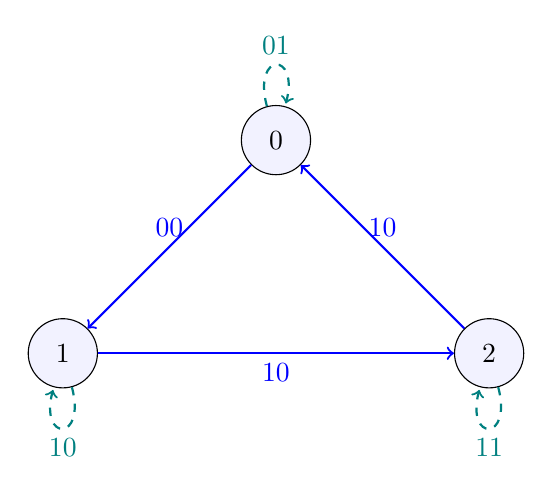
\begin{tikzpicture}

    \node[state,fill=blue!5] (x0) {$0$};
    \node[state,fill=blue!5, below left of = x0,
        yshift=-2cm, xshift=-2cm]
        (x1) {$1$};
    \node[state,fill=blue!5, below right of = x0,
        yshift=-2cm, xshift=2cm]
        (x2) {$2$};

    \draw[->,blue,thick] (x0) edge[above]
        node{$00$} (x1);
    \draw[->,blue,thick] (x1) edge[below]
        node{$10$} (x2);
    \draw[->,blue,thick] (x2) edge[above] node{$10$} (x0);

    \draw[->,dashed,teal,thick] (x0) edge[loop above]
        node{$01$} (x0);
    \draw[->,dashed,teal,thick] (x1) edge[loop below]
        node{$10$} (x1);
    \draw[->,dashed,teal,thick] (x2) edge[loop below]
        node{$11$} (x2);
        \end{tikzpicture}
\caption{Problem~\ref{prob:viterbi}.
FSM representation of an encoder with three states
$x[t]\in \{0,1,2\}$.
The solid blue lines are the transitions for $b[t]=1$,
and the dashed teal lines are the transitions for $b[t]=0$.
}
\label{fig:threestate}
\end{figure}


\end{enumerate}
\end{document}



